
\documentclass{vgtc}                          % final (conference style)
%\documentclass[review]{vgtc}                 % review
%\documentclass[widereview]{vgtc}             % wide-spaced review
%\documentclass[preprint]{vgtc}               % preprint
%\documentclass[electronic]{vgtc}             % electronic version

\usepackage{mathptmx}
\usepackage{graphicx}
\usepackage{times}
\usepackage{url}

%% We encourage the use of mathptmx for consistent usage of times font
%% throughout the proceedings. However, if you encounter conflicts
%% with other math-related packages, you may want to disable it.

%% If you are submitting a paper to a conference for review with a double
%% blind reviewing process, please replace the value ``0'' below with your
%% OnlineID. Otherwise, you may safely leave it at ``0''.
\onlineid{0}

%% declare the category of your paper, only shown in review mode
\vgtccategory{Research}

%% allow for this line if you want the electronic option to work properly
\vgtcinsertpkg

%% In preprint mode you may define your own headline.
%\preprinttext{To appear in an IEEE VGTC sponsored conference.}

%% Paper title.

\title{Interactive Multiplots For Comparing Coverage Effectiveness}

%% Author and Affiliation (multiple authors with single affiliations).
%%\author{Roy G. Biv\thanks{e-mail: roy.g.biv@aol.com} %
%%\and Ed Grimley\thanks{e-mail:ed.grimley@aol.com} %
%%\and Martha Stewart\thanks{e-mail:martha.stewart@marthastewart.com}}
%%\affiliation{\scriptsize Martha Stewart Enterprises \\ Microsoft Research}

%% Author and Affiliation (multiple authors with multiple affiliations)
\author{Adam M. Smith\thanks{e-mail: ams292@cs.pitt.edu} %
\and Joshua J. Geiger\thanks{e-mail:jj55@cs.pitt.edu}} %
\affiliation{\scriptsize University of Pittsburgh}


\abstract{Software testing increases confidence in the correctness of application source code.  Using different orderings of a test suite can enable the earlier detection of defects which allows developers to start fixing them sooner.  Finding the best ordering is difficult and there are many approaches that prioritize the ordering, resulting in many possible test suite orderings to choose from.  This paper presents a tool that allows the user to visually examine  the results of several test suite prioritization techniques and to use interaction to gain insights about the properties of the test suite and its different orders. }

%% ACM Computing Classification System (CCS). 
%% See <http://www.acm.org/class/1998/> for details.
%% The ``\CCScat'' command takes four arguments.

%%\CCScatlist{ 
 %% \CCScat{K.6.1}{Management of Computing and Information Systems}%
%%{Project and People Management}{Life Cycle};
%%  \CCScat{K.7.m}{The Computing Profession}{Miscellaneous}{Ethics}
%%}

%% Copyright space is enabled by default as required by guidelines.
%% It is disabled by the 'review' option or via the following command:
% \nocopyrightspace

%%%%%%%%%%%%%%%%%%%%%%%%%%%%%%%%%%%%%%%%%%%%%%%%%%%%%%%%%%%%%%%%
%%%%%%%%%%%%%%%%%%%%%% START OF THE PAPER %%%%%%%%%%%%%%%%%%%%%%
%%%%%%%%%%%%%%%%%%%%%%%%%%%%%%%%%%%%%%%%%%%%%%%%%%%%%%%%%%%%%%%%%

\begin{document}

%% The ``\maketitle'' command must be the first command after the
%% ``\begin{document}'' command. It prepares and prints the title block.

%% the only exception to this rule is the \firstsection command
\firstsection{Introduction}

\maketitle

%% \section{Introduction} 

Inevitably, errors are made while designing and implementing software systems. Software developers execute tests $\{t_1, t_2, t_3,\ldots, t_n\}$ in a test suite $T$ to isolate defects and gain confidence in the correctness of the code.  Each test case in the test suite exercises specific points in the system, comparing the actual output of the code to the hand computed expected one.  If a test fails, then a defect is present in the area that the test executes.  As the source code grows in size and number of features, new tests are written for the new functionality.  To ensure that the new features do not cause the system to regress, developers include every previously written test in the collection of tests.  This process of executing and re-executing the entire test suite is known as regression testing.  

Gradually, adding new tests and retaining old ones increases the size of the test suite until its execution time can become prohibitively expensive.  In some cases the regression test suite runs for several weeks \cite{empiricalfamily}.  One method of altering the test suite to resolve this issue is test suite prioritization \cite{rothermelprioritizing2001}.  Test suite prioritization attempts to find a reordering of the test cases that is more likely to locate defaults earlier in the execution of the test suite without risking the loss of coverage by removing a test.  The tests are ordered based on certain criteria that are obtained during a process called coverage monitoring.  

Coverage monitoring measures the code coverage of a test case $t_i$.  Code coverage describes any metric that enumerates specific points in the source code that are executed when a test is run, whether they are a line, a block, a method, a branch \cite{zhu}, call trees \cite{smith-calltrees} ,or some other type. Each specific program point is called a requirement.  Given a test suite $T$, coverage monitoring gives a set of requirements $R(T) = \langle r_1, r_2,\ldots,r_m \rangle$.  Each individual test $t_i$ is associated with a subset of requirements $R(t_i) \subseteq R(T)$, which it is said to \textit{cover}.  

\begin{figure}[t]
\centering
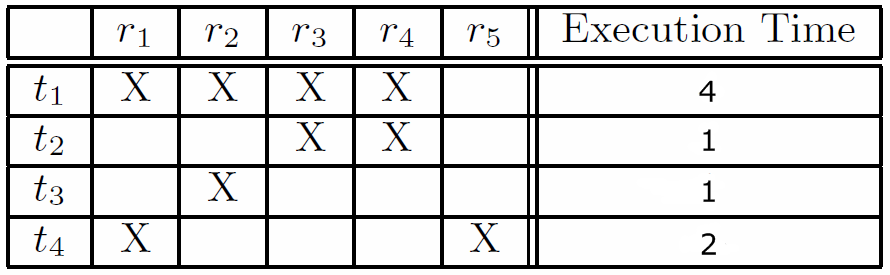
\includegraphics[scale=.2]{CoverageMatrix}
\caption{Example Test Suite}
\end{figure}
\label{fig:example}

\begin{figure}[ht]
\centering
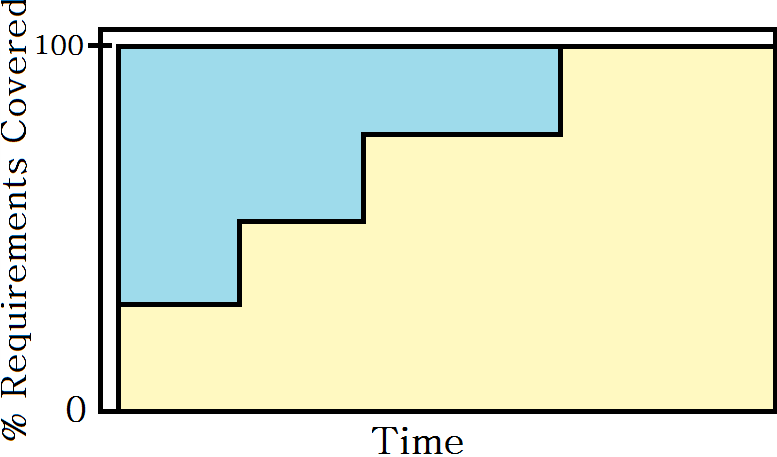
\includegraphics[scale=.2]{ce}
\caption{Coverage Effectiveness}
\end{figure}
\label{fig:ce}

Figure \ref{fig:example} shows an example of a test suite with 4 tests and 5 requirements.  An X in a cell represents that the test for that row covers the requirement in that column.  Imagine that the shown test suite is run in its original order.  In this case all of the requirements are not covered until 8 time units have passed.  Conversely, if the test suite is executed in reverse order all of the requirements are covered in 4 time units.  Covering all of the requirements sooner allows for a higher chance to find faults earlier so that the developer can more quickly begin to make changes.  

The metric coverage effectiveness (CE) \cite{ce} was developed in order to rate a test suite prioritization.  CE is derived from the step function of the cumulative coverage of a test suite as shown in Figure \ref{fig:ce}.  Each test suite offers the possibility of covering more total requirements.  When the cumulative coverage is plotted against time a step function is formed.  CE itself is calculated by dividing the area under the step function for the actual order by the area under the curve of a test suite that covers all of its requirements instantly.  This value is between 0 and 1 where 0 means that no requirements were covered, and 1 means that all of the requirements were covered instantly.

\section{Motivation}

There are a total of $n$! possible orderings of a test suite where $n$ is the number of tests.  Clearly for most test suites these cannot all be enumerated to find the highest CE.  For this reason there are several algorithmic ways to find good orderings, including random sampling.  However, it is difficult to interpret the results of several algorithms or random samples by reading text alone.  Therefore, this project aimed to create a visualization that can allow software testers to instantly see how algorithmic prioritizers perform and also to examine a set of random prioritizations simultaneously.  There is related work in the field of visualizing test suites \cite{tarantula} \cite{bart}, however, they focus on fault localization or different features of a test suite.

Examining the CE functions of several reorderings for a given test suite will reveal the effectiveness of the different prioritization techniques on that suite.  Figure \ref{fig:multi_ce} shows a multiplot of CE functions for 50 random prioritizations.  This static image does not allow for easy identification of the source of the prioritization or limiting the visualization to only prioritizations of interest.  Also, the static image cannot display qualitative data about each prioritization.  To allow for more functionality and information communication an interactive tool was developed instead of only using static images to visualize CE multiplots.

\begin{figure}[t]
\centering
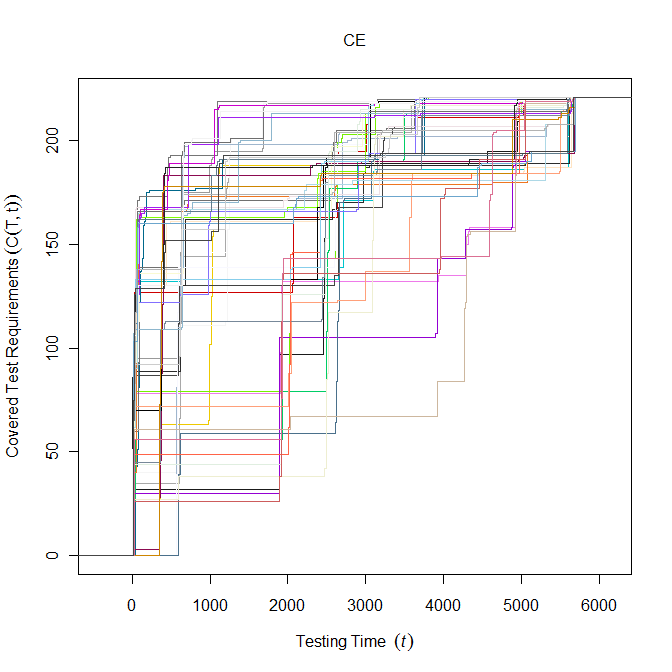
\includegraphics[scale=.25]{original}
\caption{Coverage Effectiveness Multiplot}
\end{figure}
\label{fig:multi_ce}
\section{Tool Design}

Our tool is designed to aid in analyzing multiple prioritizations of a test suite through user interaction of CE multiplots.  By providing the tool with coverage and timing data for a test suite, several prioritizations are generated using the techniques described by Smith and Kapfhammer \cite{smith:2009}.  Due to the nature of step functions consisting of only vertical and horizontal lines, plotting several functions on a single graph may obscure lines, thus making it difficult to track and compare prioritizations.  A solution to this is pruning the graph to only the plots in which the user is interested.  However, generating a new static multiplot for each comparison is cumbersome.  Therefore, in a similar approach to Becker et al. \cite{Stephen95visualizingnetwork} and a NY Times interactive visualization of market statstics \cite{nytime_multiplot} the tool allows users to interactively select techniques displayed and directly manipulate the corresponding plot.

Figure \ref{fig:screenshot} provides a screen capture of the tool showing a test suite's prioritizations.  The left panel provides data selection, while the right panel displays the multiplot.  The upper left corner gives general information on the test suite.  In this image, all techniques are currently selected to appear in the multiplot.  This is controlled by the grid of color-coded buttons which allow the user to select/deselect the prioritizations displayed.  Additionally, a mouseover of the lines of individual functions will highlight the line and shade the area under the curve, as well as, provide a label identfying the technique, parameters to the technique, and the CE value of the prioritization represented by the line.  This is superior to a static graph since the user immediately knows which prioritization the line corresponds to as well as the quality of the prioritization as determined by its CE value.  A slider on the lower left corner allows the user to generate varying numbers of random prioritizations that appear in the multiplot as thin, light gray lines.


\section{Evaluation}

Feedback on the usability and effectiveness in aiding CE comparisons of the tool was primarily provided by Dr. Gregory M. Kapfhammer, an expert in software engineering, software testing and analysis, and computer systems \cite{thehammer}.  Response to the tool was generally positive, the evaluator found the tool useful in displaying the information but made suggestions on areas where the tool could help to interpret the data.  Some suggestions include:
\begin{itemize}
 \item Displaying coverage density information
 \item Relate 'goodness' of approach (CE) through glyphs or colors
 \item Empirical cumulative distribution functions of the random
\end{itemize}
A few other suggestions on layout were also made, but our evaluator stated that the tool was already useful enough that he would use it in his own research, as well as, utilize it in teaching his future software engineering courses.  Overall, the tool met its goal of providing simple interactive technique for comparing prioritization effectiveness.

\begin{figure}
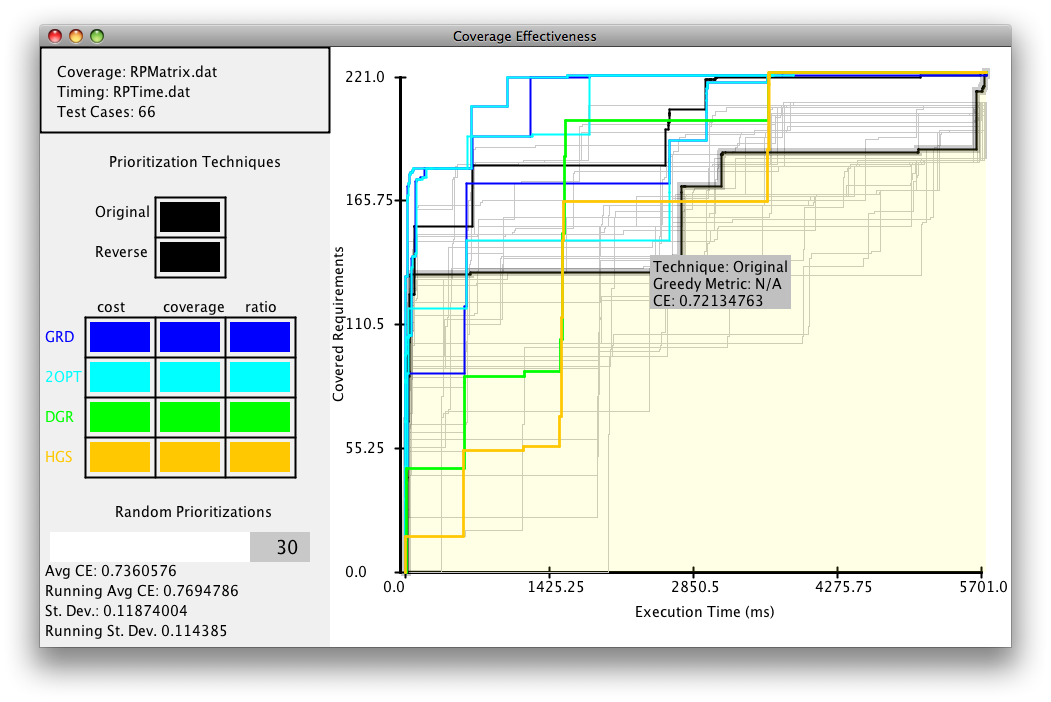
\includegraphics[scale=.25]{screenshot}
\caption{Interactive Multiplot}
\label{fig:screenshot}
\end{figure}

%% if specified like this the section will be ommitted in review mode
\acknowledgements{
The authors wish to thank Gregory Kapfhammer, Manos Renieris, and Liz Marai for assistance with this project.}

\bibliographystyle{abbrv}
%%use following if all content of bibtex file should be shown
%\nocite{*}
\bibliography{myBibtexDB}
\end{document}
